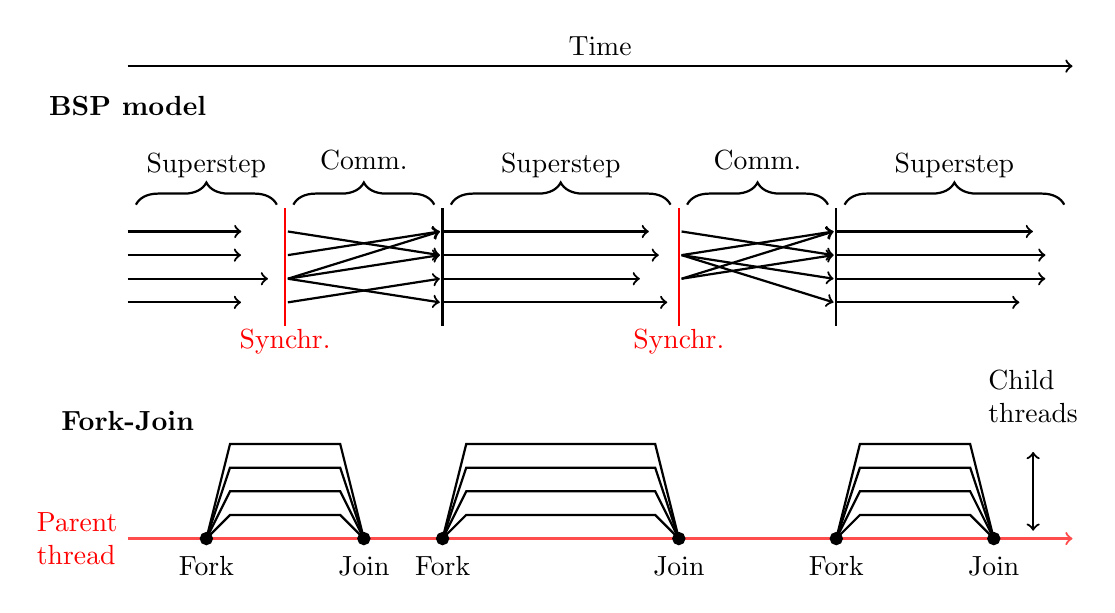
\begin{tikzpicture}[thick]
% Fork Join model
\coordinate (begin) at (0,0);
\coordinate (f0) at (1,0);
\coordinate (j0) at (3,0);

\coordinate (f1) at (4,0);
\coordinate (j1) at (7,0);

\coordinate (f2) at (9,0);
\coordinate (j2) at (11,0);

\coordinate (end) at (12,0);

\node at ([yshift=1.5cm]begin) {\textbf{Fork-Join}};


% Main threads and info
\draw[->,red!70] (0,0) -- (f0) -- (j0) -- (f1) -- (j1) -- (f2) -- (j2) -- (end);
\node[anchor=east,red,align=left] (0,0) {Parent\\thread};
\foreach \x in {0,...,2}{
\draw[fill,black,thick] (f\x) circle [radius=2pt] ;
\draw[fill,black,thick] (j\x) circle [radius=2pt] ;
\node at ([yshift=-10pt]f\x) {Fork}; 
\node at ([yshift=-10pt]j\x) {Join}; 
}

% Thread
\foreach \x in {1,...,4}{
  \draw[thick] (f0) -- ([yshift=\x*.3cm,xshift=.3cm]f0) -- ([xshift=-.3cm,yshift=\x*.3cm]j0) -- (j0);

  \draw[thick] (f1) -- ([yshift=\x*.3cm,xshift=.3cm]f1) -- ([xshift=-.3cm,yshift=\x*.3cm]j1) -- (j1);

  \draw[thick] (f2) -- ([yshift=\x*.3cm,xshift=.3cm]f2) -- ([xshift=-.3cm,yshift=\x*.3cm]j2) -- (j2);
}

% Name of threads
\draw[<->] (11.5,0.1) -- (11.5,1.1) node[anchor=south,yshift=7pt,align=left] {Child\\threads};


% BSP model
\coordinate (begin) at (0,3);

\coordinate (s0) at (2,3);
\coordinate (c0) at (4,3);
\coordinate (s1) at (7,3);
\coordinate (c1) at (9,3);
%\coordinate (s2) at (9,3);

\coordinate (end) at (12,3);

% Figure name 
\node at ([yshift=2.5cm]begin) {\textbf{BSP model}};

\draw [decorate,decoration={brace,amplitude=8pt,raise=4pt},yshift=0pt] ([yshift=1.1cm,xshift=3pt]begin) -- ([yshift=1.1cm,,xshift=-3pt]s0) node [black,midway,above,yshift=10pt] {Superstep};

\draw [decorate,decoration={brace,amplitude=8pt,raise=4pt},yshift=0pt] ([yshift=1.1cm,xshift=3pt]s0) -- ([yshift=1.1cm,,xshift=-3pt]c0) node [black,midway,above,yshift=13pt] {Comm.};

\draw [decorate,decoration={brace,amplitude=8pt,raise=4pt},yshift=0pt] ([yshift=1.1cm,xshift=3pt]c0) -- ([yshift=1.1cm,,xshift=-3pt]s1) node [black,midway,above,yshift=10pt] {Superstep};

\draw [decorate,decoration={brace,amplitude=8pt,raise=4pt},yshift=0pt] ([yshift=1.1cm,xshift=3pt]s1) -- ([yshift=1.1cm,,xshift=-3pt]c1) node [black,midway,above,yshift=13pt] {Comm.};

\draw [decorate,decoration={brace,amplitude=8pt,raise=4pt},yshift=0pt] ([yshift=1.1cm,xshift=3pt]c1) -- ([yshift=1.1cm,,xshift=-3pt]end) node [black,midway,above,yshift=10pt] {Superstep};


% Draw vertical lines 
\foreach \x in {0,...,1}{
\draw[red] ([yshift=-.3cm]s\x) -- ([yshift=1.2cm]s\x);
\node[red] at ([yshift=-.5cm]s\x) {Synchr.};

\draw ([yshift=-.3cm]c\x) -- ([yshift=1.2cm]c\x);
%\node at ([yshift=-.5cm]s\x) {Synchr.};
}

\foreach \x in {0,...,3}{
  \draw[->] ([yshift=\x*.3cm]begin) -- ([yshift=\x*.3cm,xshift=((rnd)*-20pt-2pt)]s0);
  \draw[->] ([yshift=\x*.3cm]c0) -- ([yshift=\x*.3cm,xshift=((rnd)*-20pt)-2pt]s1);
  \draw[->] ([yshift=\x*.3cm]c1) -- ([yshift=\x*.3cm,xshift=((rnd)*-20pt)-2pt]end);
  %\draw[->] ([yshift=\x*.3cm]s2) -- ([yshift=\x*.3cm,xshift=((rnd)*-20pt)-2pt]end);
}

% Add comms 
% comm 0 
\draw[->] ([xshift=1pt,yshift=.3cm]s0) -- ([xshift=-1pt,yshift=.9cm]c0);
\draw[->] ([xshift=1pt,yshift=0]s0) -- ([xshift=-1pt,yshift=.3cm]c0);
\draw[->] ([xshift=1pt,yshift=.3cm]s0) -- ([xshift=-1pt,yshift=0]c0);
\draw[->] ([xshift=1pt,yshift=.6cm]s0) -- ([xshift=-1pt,yshift=.9cm]c0);
\draw[->] ([xshift=1pt,yshift=.3cm]s0) -- ([xshift=-1pt,yshift=.6cm]c0);
\draw[->] ([xshift=1pt,yshift=.9cm]s0) -- ([xshift=-1pt,yshift=.6cm]c0);

% comm 1
\draw[->] ([xshift=1pt,yshift=.6cm]s1) -- ([xshift=-1pt,yshift=.9cm]c1);
\draw[->] ([xshift=1pt,yshift=.6cm]s1) -- ([xshift=-1pt,yshift=.3cm]c1);
\draw[->] ([xshift=1pt,yshift=.6cm]s1) -- ([xshift=-1pt,yshift=0]c1);
\draw[->] ([xshift=1pt,yshift=.3cm]s1) -- ([xshift=-1pt,yshift=.9cm]c1);
\draw[->] ([xshift=1pt,yshift=.3cm]s1) -- ([xshift=-1pt,yshift=.6cm]c1);
\draw[->] ([xshift=1pt,yshift=.9cm]s1) -- ([xshift=-1pt,yshift=.6cm]c1);


% Time 
\draw[->] ([yshift=3cm]begin) -- ([yshift=3cm]end) node[midway,above] {Time};

\end{tikzpicture}